%
\documentclass[12pt,notitlepage]{article}
\usepackage{amssymb}
\usepackage{amsmath}
\usepackage{graphicx}
\usepackage{epstopdf}
\usepackage{pdflscape}
\usepackage[pdftex,dvipsnames]{xcolor}  
\setlength{\marginparwidth}{2cm}
\usepackage[colorinlistoftodos,prependcaption,textsize=small]{todonotes}
\usepackage{xargs}
\usepackage{tabularx}
\usepackage{longtable}
\usepackage{array}
\usepackage{dsfont}
\usepackage{float}
\usepackage{booktabs}
\usepackage{tikz}
\usepackage{marvosym}
\usepackage{multirow}
\usepackage{pdflscape}
\usepackage[hyphens]{url}
\usepackage{setspace}
\usepackage{epigraph}
\usepackage{bm}
\usepackage{textcomp}
\usepackage{diagbox}
\usepackage{bbm}
\usepackage{verbatim}
\usepackage[framemethod=tikz]{mdframed}
\usepackage{subcaption}
\usepackage{caption}
\usepackage{lipsum}
\usepackage{mathtools}
\usepackage{scalerel}
\usepackage{stackengine}
\usepackage{amsthm}
\usepackage{epsfig}
\usepackage[
backend=bibtex,
style=authoryear-comp,
sorting=ynt
]{biblatex}
\usepackage[colorlinks,allcolors=blue]{hyperref}
\usepackage[shortlabels]{enumitem}
\usepackage{subfiles} % Best loaded last in the preamble


\setlength{\epigraphrule}{0pt}
\renewcommand{\baselinestretch}{1.25}

\setcounter{MaxMatrixCols}{10}

\newcolumntype{L}[1]{>{\raggedright\let\newline\\\arraybackslash\hspace{0pt}}m{#1}}
\newcolumntype{C}[1]{>{\centering\let\newline\\\arraybackslash\hspace{0pt}}m{#1}}



\newcommand{\I}{\mathbb{I}}
\newcommand{\E}{\mathbb{E}}
\newcommand{\Ll}{\mathrm{L}}
\newcommand{\R}{\mathbb{R}}
\renewcommand{\L}{\mathbb{L}}
\newcommand{\Var}{\mathrm{Var}}
\newcommand{\Cov}{\mathrm{Cov}}
\newcommand{\Corr}{\mathrm{Corr}}
\newcommand{\Prob}{\mathbb{P}}
\newcommand{\supp}{\mathrm{supp}}
\newcommand{\notimplies}{\mathrel{{\ooalign{\hidewidth$\not\phantom{=}$\hidewidth\cr$\implies$}}}}
\newcommand{\var}{\mathrm{var}}
\newcommand{\Bias}{\mathrm{Bias}}
\newcommand{\cov}{\mathrm{cov}}
\newcommand{\corr}{\mathrm{corr}}
\newcommand{\MSE}{\mathrm{MSE}}
\let\OldTodo\todo
\RenewDocumentCommand{\todo}{O{} m}{\OldTodo[#1]{\textbf{TODO}: #2}}
\newcommandx{\thiswillnotshow}[2][1=]{\OldTodo[disable,#1]{#2}}
\newcommandx{\askjesse}[2][1=]{\OldTodo[linecolor=Plum,backgroundcolor=Plum!25,bordercolor=Plum,#1]{\textbf{{Ask Jesse:}} #2}}
\newcommandx{\longterm}[2][1=]{\OldTodo[linecolor=Blue,backgroundcolor=Blue!25,bordercolor=Blue,#1]{\textbf{{Long-term:}} #2}}
\newcommandx{\takeaway}[2][1=]{\OldTodo[linecolor=Green,backgroundcolor=Green!25,bordercolor=Green,#1]{\textbf{{Takeaways:}} #2}}


\topmargin=-1.5cm \textheight=23cm \oddsidemargin=0.5cm
\evensidemargin=0.5cm \textwidth=15.5cm

\newtheorem{theorem1}{Special Theorem}

\newtheorem{ass}{Assumption}
\newtheorem{definit}{Definition}
\newtheorem{prop}{Proposition}
\newtheorem{thm}{Theorem}
\newtheorem{lem}{Lemma}
\newtheorem{conj}{Conjecture}
\newtheorem{cor}{Corollary}
\newtheorem{rem}{Remark}

\renewcommand{\thesubsection}{\arabic{section}.\arabic{subsection}}
\renewcommand{\thesubsubsection}{\arabic{section}.\arabic{subsection}.\arabic{subsubsection}}

\newcommand\dapprox{\stackrel{\mathclap{\tiny \mbox{d}}}{\approx}}
\newcommand\papprox{\stackrel{\mathclap{\tiny \mbox{p}}}{\approx}}
\newcommand\pconverge{\stackrel{\mathclap{\tiny \mbox{p}}}{\to}}
\newcommand\dconverge{\stackrel{\mathclap{\tiny \mbox{d}}}{\to}}

\addbibresource{source/paper/references.bib}


\newcommand\independent{\protect\mathpalette{\protect\independenT}{\perp}}
\def\independenT#1#2{\mathrel{\rlap{$#1#2$}\mkern2mu{#1#2}}}

\onehalfspacing
\newtheorem{theorem}{Theorem}
\newtheorem{corollary}[theorem]{Corollary}
\newtheorem{proposition}{Proposition}

\newtheorem{hyp}{Hypothesis}
\newtheorem{subhyp}{Hypothesis}[hyp]
\renewcommand{\thesubhyp}{\thehyp\alph{subhyp}}

\newcommand{\red}[1]{{\color{red} #1}}
\newcommand{\blue}[1]{{\color{blue} #1}}

\newcolumntype{L}[1]{>{\raggedright\let\newline\\arraybackslash\hspace{0pt}}m{#1}}
\newcolumntype{C}[1]{>{\centering\let\newline\\arraybackslash\hspace{0pt}}m{#1}}
\newcolumntype{R}[1]{>{\raggedleft\let\newline\\arraybackslash\hspace{0pt}}m{#1}}

\begin{document}

\begin{titlepage}
\title{Collaboration in Organizations: Evidence from Open Source Software}
\author{Christopher Liao

\thanks{I am indebted to my advisors Jesse Shapiro and Ali Hortaçsu. I thank Jordan Rosenthal-Kay, James Traina, Noah Sobel-Lewin, Krishna Dasari, Anjali Pullabhotla, Luis Garicano, Josh Lerner, Frank Nagel, Victor Lima, Kotaro Yoshida, Jeff Gortmaker, Ruru Hoong, Ruby Zhang and Matthew Lee Chen, and members of the Harvard Predoc Workshop and the UChicago Honors Workshop for helpful comments and suggestions.}

\date{\today}
\maketitle
\begin{abstract}
\noindent Placeholder\\
\vspace{0in}\\
\noindent\textbf{Keywords:} key1, key2, key3\\

\bigskip
\end{abstract}
\setcounter{page}{0}
\thispagestyle{empty}
\end{titlepage}
\pagebreak \newpage

\section{Introduction} \label{sec:intro}

\todo[inline]{To do's for the introduction\\
2) Rewrite motivation to emphasize organizational resilience as the thing we don't know\\
5) Rewrite methods to suit what I'm currently doing\\
6) Rewrite findings\\
7) Write literature – understand what the literature has done}

\textbf{Paragraphs 1-2: Motivation. After reading these paragraphs a reader in any field of economics should believe that if you answer your research question your paper will make an important contribution.}
\todo[inline]{
1. Evaluate whether I need to just focus on collaboration (depends on whether/how I incorporate communication)\\
2. Is knowledge loss a useful term\\
3. Think about whether there's an angle to describe "we don't know how organizations benefit from collaboration". I could approach it from a pre-post departure tradeoffs angle, a "what types of projects benefit most", "what types of departures benefit most", or a "the different opposing forces" angle. 
4. Is there a way to incorporate the model of hierarchy and how it doesn't tell us about collaboration?
}


A key issue organizations encounter is departures. \todo[inline]{Is there a citation I can use to characterize the costs of collaboration?}
An organization's problem-solving ability depends on the knowledge of its contributors; hence, departures can not only lead to less hands on deck, but also the shrinking of the organization's knowledge base and problem-solving ability. Oftentimes, the more important the departed contributor, the greater the repercussions. One way organizations can mitigate the repercussions of departures is through collaboration. Collaboration can expose contributors to a wider variety of tasks, allowing collaborators to expand their own knowledge base through learning from others and limit how much knowledge an organization would lose following a departure (\cite{hamilton_team_2003}, \cite{rashid_systematic_2019}). On the other hand, collaboration might also lead to investments in team-specific capital that are inaccessible and ill-fitted for the organization's broader objectives post-departure, negatively affecting collaborators (\cite{jaravel_team-specific_2018}, \cite{azoulay_does_2019}). \todo[inline]{Should I be worried about the fact that I'm giving examples I can't really test?} Moreover, collaboration can also create organizational burdens, as collaboration involves repeating information, dealing with scheduling frictions and learning about new problems, all of which are time consuming and can detract from the organization's primary focus. \todo[inline]{I want to amend "repeating information, dealing with scheduling frictions and learning about new problems" based off what I find to be time consuming in the paper} In this paper, my goal is to understand whether collaboration is effective in mitigating the repercussions of important departures in organizations and the tradeoffs associated with collaboration. \todo[inline]{1. I'm not sure if I want to mention tradeoffs if it's not a major portion of my analysis and 2. Do I want to try and put tradeoffs on the same scale as impacts?}


\todo[inline]{Consider whether to change contributors with members}

\textbf{Paragraphs 3-4: Challenges. These paragraphs explain why your research question has not already been answered, i.e., what are the central challenges a researcher must tackle to answer this question.}

There are two major challenges that must be addressed to assess how collaboration affects projects following the departure of an important contributor. First, granular data about organizations is typically inaccessible to researchers. Second, departures and an organization's collaborative nature are both endogenous, which makes identifying their causal effect on an organization difficult. 

I address the first challenge by studying organizational departures using evidence from open source software (OSS) development organizations. OSS is software that is freely available for use and modification, and is considered a public good. OSS is widely used - a recent report found that 97\% of all software included open source code (\cite{fred_bals_six_2025}). Prominent examples of OSS projects include the operating system Linux, the operating system of choice for 96.4\% of the top one million web servers (\cite{w3cook_os_2015})\footnote{Ubuntu, CentOS, Debian, Fedora, SUSE and Redhat are all Linux-based}, and the machine learning framework PyTorch, which is used by 63\% of all organizations training artificial intelligence/machine learning models (\cite{lawson_shaping_2024}). \todo[inline]{Add Python}

Granular OSS development activity is publicly available for research. Moreover, concerns about the repercussions of departures are particularly acute in the OSS community as most contributors are mostly volunteers (\cite{robles_evolution_2005}, \cite{xu_volunteers_2010}) which leads to high turnover (\cite{izquierdo-cortazar_using_2009}, \cite{rashid_systematic_2019}). Past research has found that departures negatively affect software quality (\cite{mockus_organizational_2010}; \cite{foucault_impact_2015}).

Identifying the causal effect of departures on organizations and the causal effect of collaboration on mitigating the repercussions of departures is difficult because departure and collaboration are choices made by individual contributors and the organization. Contributor departure can occur for personal reasons unobservable to the researcher, such as personal dissatisfaction with the project (\cite{hannon_retaining_2008}, \cite{yu_empirical_2012}) or employment changes (\cite{miller_why_2019}), that may be related to underlying trends in organizational outcomes. Similarly, projects may choose to be more collaborative because collaboration is more conducive to success in their problem environment or contributors happen to enjoy working together. A naive analysis would risk confounding differences in a project's problem environment or its contributor's personalities with the actual effect of collaboration. 

\todo[inline]{Consider adding smth about how at companies that develop OSS there's high turnover}

\textbf{Paragraph 5: This Paper. This paragraph states in a nutshell what the paper accomplishes and how. }

In this paper, I leverage data on open source software to identify a set of plausibly exogenous important departures and quantify the effects of these departures on OSS projects. I analyze how pre-departure organizational characteristics affect software development activity and extend these results to characterize the impacts on downstream business outcomes. Finally, I probe at the underlying mechanisms that drive collaboration's effect and characterize tradeoffs that collaborative organizations encounter prior to departures. 

\todo[inline]{Return to this once I finish the paper}
\todo[inline]{Think more about the way I can deploy random forest (throughout the rest of the paper, before incorporating here). Is the benefit of the random forest to help with hypothesis generation for what factors mitigate departures? Or to better probe at the effects of departures}

\longterm[inline]{Paragraphs 6-7: Model. Summarize the key formal assumptions you will maintain in your analysis.

Per discussion with Jesse, I can include a model if it makes mechanisms easier to explain. }
% formal model

\iffalse
Paragraph 4 (if I end up having time to write a model): 
Model of hierarchy incorporates cooperation and communication as key features of the hierarchy that affect downstream project outcomes. However, we take these for granted and irl, communication and cooperation can't be taken for granted
\begin{enumerate}
    \item Extent of communication 
    \item Degree of cooperation, overlap (clustering)
\end{enumerate}

Existing theory tells us how organizations adapt their organizational structure and strategy in response to external shocks. However, it doesn't tell us how that adaption depends on existing organizational structure. One example: communication is an integral part of how an organization solves problems, but we don't model how it occurs. Moreover, communication itself also has pros and cons - does it have a positive effect by sharing knowledge or negative effect by creating reliance and thus inhibiting learning?

% See https://www.sciencedirect.com/science/article/abs/pii/S0268401217310095 for a survey of current work
- Doesn't try to separate relationship between structure and departures
- Does not consider the complementarity of organizational structure 
- Research on impact of organizational structures only provides suggestive evidence on the mechanism by which organizational structures have impacts. 
- The focus of research has been on codebase related outcomes or "project survival" as opposed to more relevant outcomes such as usage. 
\fi 

\textbf{Paragraphs 8-9: Data. Explain where you obtain your data and how you measure the concepts that
are central to your study}
I obtain data on OSS organizations and their software development activity from the Github Archive (\cite{github_archive_github_2025}). My paper hones in on a particular type of OSS organization - those developing widely used\footnote{I define widely used as those with at least 1000 monthly downloads each month from September 2018 to July 2023} Python libraries - because data on usage and software version updates is available through the Python Package Index \todo[inline]{Cite}. Python libraries are collections of pre-written software that provide a diverse range of functionality and are essential to software development in Python, the world's most widely used programming language as of July 2025 (\cite{paul_jansen_tiobe_2025}). The action-level data from the Github Archive (\cite{github_archive_github_2025}) allow me to identify important contributors and track their contribution and departure patterns. 

\todo[inline]{Do I need more detail? }

\textbf{Paragraphs 10-11: Methods. Explain how you take your model to the data and how you overcome the
challenges you raised in paragraphs 3-4.}

I identify a set of important departures that are unrelated to unobservable organizational trends by examining the effect of abrupt departures. Abrupt departures occur when an important contributor is highly active for several consecutive periods until their departure, afterwhich they cease to ever be involved in the organization in any capacity. The literature has found that abrupt departures tend to be driven by external shocks unrelated to the project, such as job changes or major life events, rather than internal or project-related factors such as declining interest, dissatisfaction, or project wind-down, which typically involve gradual disengagement  \cite{miller_why_2019}. 

I estimate the empirical effect of important departures using an event study design. My observations are at the organization level and the treatment date is the time period of the important departure. The control group consists of not-yet-treated projects that eventually experience a single departure, which guards against bias introduced by unobserved differences between projects that do and do not undergo departures. To simplify the identification of dynamic effects, I restrict the sample to organizations that only ever experienced a single important departure, so that the treatment is binary and irreversible. My primary estimation method is \cite{callaway_difference--differences_2021}. 

\todo[inline]{Improve this paragraph. Broadly I'm thinking something like this:
Add sentences below after I ensure I'm actually executing those tasks:
1. I define collaboration as joint involvement in problem solving between the departed contributor and other key contributors, and I show that my measure of collaboration is unrelated to measures of broader organization-wide collaboration. 
2. To ensure that collaboration with other key contributors is an option, I only include OSS organizations that have multiple key contributors in all preperiods. 
3. Finally, among {x, y, z} dimension, projects with collaborative departed contributors are observably similar to projects with uncollaborative departed contributors. 
- Also think about how I can show that collaborative projects are observably similar to uncollaborative projects??
}

\if
% does the miller paper describe "abrupt"
Quotes from Miller 2019
 One such blog post describes how “as [my project’s] pop-
ularity rose and rose, my drive to continue to create new projects, fell. All while the
burden of supporting the needs of the massive user bases of my successful projects and
the pressure of maintaining those projects grew.”

Also, Miller 2019 use abrupt engagement and finds different results from other papers
\fi

\textbf{Paragraphs 12-13: Findings. Describe the key findings. Make sure they connect clearly to the motiva-
tion in paragraphs 1-2.}
\todo[inline]{Here, outline both what I've already found and what I'm hoping to find so I have a better sense of next step}

\begin{enumerate}
    \item Departures matter
    \todo[inline]{a. How do they affect downstream outcomes (releases, downloads)? \\
    b. Do they affect other outcomes as well, such as discussion (issues opened/comments, willingness to contribute (fork))}
    \item Collaboration with the departed does affect post-departure dynamics. Surprisingly, collaborative projects perform worse. 
    \item Involvement matters. The most involved departed contributor belongs to the project whose post-departure outcomes were worse
    \item Collaboration has large positive benefits for the most involved group. This occurs because in collaborative projects, contributors who were already present increase their productivity. 
    \textcolor{red}{
        \begin{itemize}
            \item Why do those contributors increase their productivity? Think about this from the perspective of what this teaches us about organizations
            \begin{itemize}
                \item Is collaboration with the departed contributor indicative of broader, project-specific trends? How: Examine "other collaboration"
                \item How are the key contributor(s) they work with affected? We would suspect these individuals either benefit most (or suffer most)
                \begin{itemize}
                    \item Use this to segway into better understanding what's going on with communication. 
                \end{itemize}
                \item How can I measure whether "collaborators" are learning?
                \begin{itemize}
                    \item Do collaborators tend to work on more problem types (with and without the contributor)? Do they work on a more diverse set of things compared to others in uncollaborative projects? How does this effect change over time. Does this have an effect on outcomes?
                    \item Does a more long-term collaboration help (time)? What about having collaborated on many problems together?
                    \item Do they engage in other forms of responsibility more often, such as reviewing PRs, closing issues, commenting on other's issues? Does this have an effect on outcomes?
                    \item Are they able to do more things independently (either because the departed contributor isn't involved, or becomes less involved) throughout the duration of their collaboration? Does this have an effect on outcomes?
                \end{itemize}
                \item What are the tradeoffs associated with collaboration? Do the tradeoffs affect post-departure outcomes in any way?
            \end{itemize}
        \end{itemize}
    }
    \item Collaboration has large negative benefits for all other involved groups. This occurs because in collaborative projects, contributors who were already present leave. 
    \textcolor{red}{
    \begin{itemize}
            \item Why do those contributors leave? Think about this from the perspective of what this teaches us about organizations
            \item Are the ones who are leaving the key contributor collaborators? 
        \end{itemize}
    }
    \item New contributors are very productive, even more so than existing ones. Why?
\end{enumerate}


\todo[inline]{It would be nice to place a number on "impacts"}
% I also want a robustness for departures (that are vs. aren't abrupt) using that departure filtering event study graph

\textbf{Paragraphs 14-15: Literature. Lay out the two main ways your paper contributes to the literature. Each paragraph should center around one contribution and should explain precisely how your paper differs from the most closely related recent work.}
\textbf{approach wil be to write down strands of related literature and return to this once I'm done }

I think it applies to two literature
\begin{enumerate}
    \item Literature on OSS in economics: no one has thought about departures, rare to see big data deployed. Literature on OSS doesn't address endogeneous nature of departures or org structure well 
    \item Literature on org/team structure: how do org characteristics affect outcomes. In economics, there's the theory (Brynjolfsson, Milgrom - complementary org structures), applications to management (Bloom) and evidence from the inventor literature (Azoulay, Jaravel)
\end{enumerate}


\todo[inline]{Ensure that each sentence in each section of the introduction clearly maps to a theme/subsection of the paper}

\section{Data} \label{sec:data}
\longterm[inline]{I may want to think about data as data sources, and data definitions}
\todo[inline]{When I return to this, first think about the big pieces, then match what I've already written to the big pieces/what still needs to be filled in for the big pieces, and then write}
\begin{enumerate}
    \item What is an open source software project (unit of measurement)?.
    \begin{itemize}
        \item Appendix: How I map PyPi projects to github repositories
        \item Appendix: How I match repo names to repo ids in cases where identity changes
    \end{itemize}
    \item Who are contributors and how do contributors contribute to the project (describe a "problem unit")?
    \begin{itemize}
        \item Describe the many purposes of an issue and define the key concepts in an issue thread. Add a screenshot to help inform what these are like
        \item Describe the purpose of a PR, and define the key concepts in a PR thread. Add a screenshot to help inform what these are like. 
        \begin{itemize}
            \item Appendix: How I measure PRs merged and other related concepts (is it a subset of opened PRs?)
        \end{itemize}
        \item Units of code change: commits, which come from pushes + PRs. 
        \begin{itemize}
            \item Appendix: How are commits measured and deal with the fact that push and PR commits can be overlapping? 
        \end{itemize}
    \end{itemize}
    \item Measurement of downstream outcomes - the deifne the ones that I end up using. 
    \begin{itemize}
        \item Describe software releases, the various types and measurement
        \item Define software quality (security measure, not user experience based)
        \item Downloads
    \end{itemize}
    \item Measurement: Aggregation to the 6 month level
    \begin{itemize}
        \item Appendix: Robustness to 3 month measurements (if necessary)
    \end{itemize}
    \item Appendix: Data availability (when is it first available, what is the availability rate)
\end{enumerate}
\todo[inline]{I think define problems first, then define departure, then define organizational structure. along the way define the different splits I use. }
\subsection{Measuring Departure}
\begin{enumerate}
    \item Subset of contributors whose code contributions were above the 75th percentile for at least 3 consecutive periods before
    \item Commits declined immediately to 0 in the "departure" period
    \item Departure is permanent
    \item Departure means all other activities in all other areas ceases too 
    \todo[inline]{check if this zero activity rule applies starting the departure period or period after departure}
    \item Project only experienced one departure. 
\end{enumerate}
\subsection{Measuring Organizational Structure}
The key ingredients needed are a definition of key contributor and  problems the project solves. 
\subsubsection{Defining key contributors}
\begin{enumerate}
    \item Construct a network of interactions between contributors based off issue threads, PR threads and PR review threads.
    \begin{itemize}
        \item Include example
    \end{itemize}
    \item Mark contributor as key if they meet either one of the two criteria in any of the past 3 time periods \textbf{AND} they're still active
    \begin{enumerate}
        \item their degree (number of nodes they were connected to) z score exceeded 1.5 or had the highest z score 
        \item they are the departed contributor
    \end{enumerate} 
\end{enumerate}
\subsubsection{Defining the set of problems}
\begin{enumerate}
    \item First construct a mapping between issues + PRs. This helps create a dataset of "problems" that projects address
    \begin{itemize}
        \item Three problem types: unlinked issues, unlinked PRs, linked
        \item Construct linkage using the following criteria
        \begin{enumerate}
          \item Use the provided link.
          \item For each remaining unlinked issue/PR, find a counterpart that mutually references it and choose the closest number.
          \item If no mutual reference exists, find any one-way reference and choose the closest number
        \end{enumerate}
    \end{itemize}
    \item Only keep projects that have at least two key contributors in all pre-treatment periods (henceforth known as pre periods)
\end{enumerate}
\subsubsection{Defining collaboration}
For a given project $i$ in time period $t$, and problems $P_{it} = \{p_{it}^1, \cdots, p_{it}^{N_{it}} \}$ where $N_{it}$ is the number of problems faced by project $i$ in time period $t$
\begin{itemize}
    \item Let $C_{it}$ denote the set of all contributors to project $i$ in time $t$. We can decompose all contributors into key and other contributors: $C_{it} = C_{it}^{key} \cup C_{it}^{other}$ 
    \item For each problem $p_{it}^k$ you have a set of collaborators $C_{it}^{k} \subseteq C_{it}^{key} $ that consists of key ($C_{it}^{k, key} = C_{it}^{k} \cap C_{it}^{key}$) and other collaborators ($C_{it}^{k, other} = C_{it}^{k} \cap C_{it}^{other}$)
\end{itemize}
Define collaboration as when 2 or more key contributors are both involved in a problem and the collaboration score
\begin{equation}
    CollabScore_{it} = \frac{1}{N_{it}}\sum_{k=1}^{N_{it}}\mathbf{1}\bigl\{|C_{it}^{k,\mathrm{key}}|\ge2\bigr\}
\end{equation}
This definition of collaboration has a nice decomposition. Let $P_{it}^d = \{p_{it}^{k} \mid d \in C_{it}^k, 1 \leq k \leq N_{it} \}$ be the set of problems where the departed contributor $d$ is involved and let $N_{it}^d = |P_{it}^d|$. Use the superscript $nd$ to denote problems where the departed contributor is not involved. I can describe collaboration as a weighted average of collaboration in problems where the departed contributor is and is not involved. 
\begin{align*}
    CollabScore_{it} &= \frac{N_{it}^d}{N_{it}} CollabScore_{it}^d + \frac{N_{it} - N_{it}^d}{N_{it}} CollabScore_{it}^{nd} \\
    &= \frac{N_{it}^d}{N_{it}} \frac{1}{N_{it}^d} \sum_{k \in P_{it}^d} \mathbf{1}\bigl\{|C_{it}^{k,\mathrm{key}}|\ge2\bigr\} + \frac{N_{it} - N_{it}^d}{N_{it}} \frac{1}{N_{it} - N_{it}^d} \sum_{k \notin P_{it}^d} \mathbf{1}\bigl\{|C_{it}^{k,\mathrm{key}}|\ge2\bigr\}
\end{align*}
\subsection{Sample}
All projects have at least 2 key contributors and at least 5 PRs opened in the pre period. 

\subsection{Aspirational To Dos}
\begin{enumerate}
    \item Read this  \href{https://pubs.aeaweb.org/doi/pdfplus/10.1257/jep.36.3.211}{paper} in order to understand how to motivate the paper using descriptive statistics
    \item Provide insight into what a project is like, such as
    \begin{itemize}
        \item How many people are in a project at a given point in time (can I divide it into important/unimportant people)?
        \item What are churn rates like among both hierarchies?
        \item How many problems are they solving, how much disussion is there and what solutions are proposed?
        \item What do outcomes look like for these projects?
        \item Provide estimates of data coverage at a project level     
        \item How many time periods do I have projects for
        \item How much discussion and people per problem?
    \end{itemize}
    \item Add reference to showing that results are not sensitive to changes in parameters/if they are, justify why mine is reasonable 
\end{enumerate}



\section{Methods} \label{sec:method}



\textcolor{red}{To do's
\begin{enumerate}
    \item Define notation and express ES equation
    \item What normalizations etc
    \item Discuss assumptions
    \item Discuss the interpretation of the event study coefficient
    \item Discuss how I execute the HTE and how the coefficient interpretation changes with HTE
    \item Discuss how I analyze with Wald
    \item Defend exogeneity for HTE
    \item Discuss how I execute different subsamples and 
    \item Describe power issues, how I examine downstream outcomes and the interpretation of downstream outcome coefficients
    \item Methods used for causal validation 
\end{enumerate}}
\todo[inline]{Revisit methods once I work more on results to see what's the best way to present them}

\subsection{Estimating the Effect of Contributor Departures}
Define each time period as $t \in \{1, \cdots, T\}$ where $t=1$ is INSERTEARLIESTDATE and $t=T$ is INSERTLATESTDATE. For each project $i$, let $T_i$ (where $1 < T_i < T$) denote the period of the key contributor’s $d_i$'s departure (henceforth the treatment date), and define the treatment indicator as $D_{it} = \mathbf{1}\{\,t \ge T_i\}$. A project's treatment date $T_i$ is the first time period where the departed key contributor $d_i$ is inactive in the project. 

My primary outcome $Y_{it}$ is the z-score of the number of pull requests opened by all contributors in project $i$ in time period $t$. Throughout the paper, I also consider other outcomes, which are also expressed in units of z-score. Formally, define $Y_{it}^c$ as the quantity of pull requests opened by all contributors in project $i$ in time period $t$, the pre-treatment mean as $\bar{Y}_{it}^{pre} = \frac{1}{5}\sum_{t=T_i-5}^{T_i-1} Y_{it}^c$ and pre-treatment standard deviation as $\sigma_{it}^{pre} = \frac{1}{5}\sum_{t=T_i-5}^{T_i-1} \left (Y_{it}^c - \bar{Y}_{it}^{pre} \right)^2$. Then, $Y_{it} = \frac{Y_{it}^c - \bar{Y}_{it}^{pre}}{\sigma_{it}^{pre}}$. Standardizing all projects such that the units are in standard deviations allows me to compare projects in a uniform way in spite of drastic differences in counts.  

\todo[inline]{Write theta, write how it disaggregates to g-t after i say I use CS}
If the outcome $Y_{it}$ is the z-score of pull requests opened by project $i$ in time period $t$, the parameter of interest in my setting is the causal effect of a key contributor departure on the project after $k$ periods, in units of standard deviation. 
\begin{equation}
    \theta_{k} = E[]
\end{equation}
I estimate $\theta_k$ using \cite{callaway_difference--differences_2021} because it allows for using not-yet-treated projects as the control group in my setting, which strengthens the plausibility of my identification assumptions. . 

\t
The assumptions required by \cite{callaway_difference--differences_2021} for causal identification are 
\todo[inline]{Turn into a paragraph, use math}
\begin{enumerate}
    \item No anticipation: Projects don't adjust their behavior prior to the departure date. I only use abrupt departures (which do occur in the literature), so presumably, there's little time for the project to react/adjust it's behavior
    \todo[inline]{Add literature refs on abrupt departure + context }
    \item Parallel trends: Projects that experience departures would have opened the same number of PRs had a departure not occurred. Fundamentally, the departure isn't associated with any other project changes that would affect the number of pull requests opened.
    \begin{enumerate}
        \item Abrupt departures are more likely to be unassociated with project characteristics that would endogenously affect the outcome because they're often associated with job changes. Since OSS contribution for most is a hobby, not their main career consideration, job changes are a good source of exogeneous variation because it's unlikely they're related to project related factors that make departure endogenous, but they can often disrupt contribution because the new job may prohibit or limit OSS contribution, or involve increased time that distracts from OSS 
        \todo[inline]{Add literature cites from that paper using abrupt departures, also make this more concise}
        \todo[inline]{\textbf{Show this is true}: Abrupt departures aren't associated with changes in demand for the departed contributor's services - the number of issues opened, forks, stars and downloads are still increasing. Moreover, the departure date is unrelated to the proximity to major software releases/updates}
        \todo[inline]{Can I show that organizational characteristics that might lead to dissatisfaction/change aren't the driving reason for departure/aren't systematically changing in a way that would explain their departure? For example, we don't see declines or increases in contributor count prior to their departure (signalling broad organizational changes) or changes in the distribution of communication z score/key contributors (which also suggests changes in how people are communicating/working) or in the sentiment of their communications (are they getting burnt out?)}
        \todo[inline]{Incorporate picture of the ES graph of corporate departues for my chosen specification? Highlights how many of these are corporate related}
    \end{enumerate}
\end{enumerate}

\todo[inline]{Describe what I fulfill with the assumptions}
Under the previous two assumptions, an event study estimate 

\subsection{Heterogeneous Effects}
\longterm[inline]{Random forest will help because it can deal with continuous values in a more systematic way. Right now I'm essentially assuming functional form - can think about how to phrase}
\todo[inline]{Ensure language and math is consistent with data section}
\todo[inline]{Note two nuances - there's comparing projects, and evaluating actual outcomes (relative to 0, no difference).}
\todo[inline]{Add subsubsections}

Recall that $C_{it}$ is the collaboration score of project $i$ in time period $t$, $N_{it}$ is the number of problems addressed by project $i$ at time $t$ and $I$ is the set of all projects.

Define each project’s pre-departure weighted average collaboration score $\bar C_i$,  the overall average project collaboration score $\bar C$ and project collaborativeness $C_i \in \{0, 1\}$ as

\[
\bar C_i \;=\;
\frac{\displaystyle\sum_{t=-5}^{-1} N_{it}\,C_{it}}
     {\displaystyle\sum_{t=-5}^{-1} N_{it}}
\qquad 
\bar C \;=\;
\frac{1}{\lvert I\rvert}\sum_{i\in I}\bar C_i
\qquad 
C_i = \mathbf{1}\{\bar C_i > \bar C\}
\]
I can also extend this definition to characterize project $i$'s departed contributor collaborativeness $C_i^d$ and other contributor collaborativeness $C_i^{nd}$.  
\todo[inline]{Define uncollaborativeness}

To compare statistically how collaborative and uncollaborative projects perform post-departure, I can use a Wald test. First, I estimate separate event study estimates for collaborative and uncollaborative projects. 

I will be testing whether the difference in event study coefficients  

To assess whether two project types are affected differently by departure, I conduct a Wald test on whether the difference in event study coefficients during the period of departure and the 5 periods after are different from zero. More precisely, let the event study coefficients for collaborative projects $\hat{\boldsymbol\theta}^{(c)}$, uncollaborative projects $\hat{\boldsymbol\theta}^{(u)}$ and their diference from $t=0$ to $t=5$ be defined as
\[
  \hat{\boldsymbol\theta}^{(c)}
    = \bigl(\hat\theta^{(c)}_{0},\,\hat\theta^{(c)}_{1},\,\dots,\,\hat\theta^{(c)}_{5}\bigr)^{\!\top}
  \quad
  \hat{\boldsymbol\theta}^{(u)}
    = \bigl(\hat\theta^{(u)}_{0},\,\hat\theta^{(u)}_{1},\,\dots,\,\hat\theta^{(u)}_{5}\bigr)^{\!\top}
    \qquad 
  \Delta = \hat{\boldsymbol\theta}^{(c)} - \hat{\boldsymbol\theta}^{(u)}
\]

My null hypothesis is \[
H_0: \Delta = \mathbf{0}
\]

For expositional clarity, I define the short‐term treatment effects as the event‐study coefficients in the first three post‐departure periods,
$\{\hat\theta_{0},\hat\theta_{1},\,\hat\theta_{2},\,\hat\theta_{3}\}$ 
and the long-term effects as those in the fourth period and beyond. 

\todo[inline]{Define what it means for a contributor to be more or less involved. }


\section{Results} \label{sec:result}
\todo[inline]{Describe, in more detail, how to interpret one of the graphs. }
\todo[inline]{I feel like there's not enough analysis and too much graph interpretation. I think we can improve this by moving information to the figure notes and outlining more what I want to gain from the paper}
\begin{figure}[htbp]
    \centering
    \begin{minipage}[b]{0.49\textwidth}
        \centering
        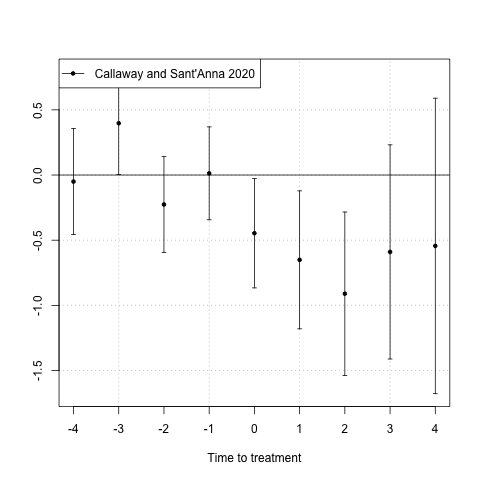
\includegraphics[width=\textwidth]{temp/output/prs_opened_norm.png}
        \subcaption{All projects}
        \label{fig:all_prs_opened}
    \end{minipage}
    \hfill
    \begin{minipage}[b]{0.49\textwidth}
        \centering
        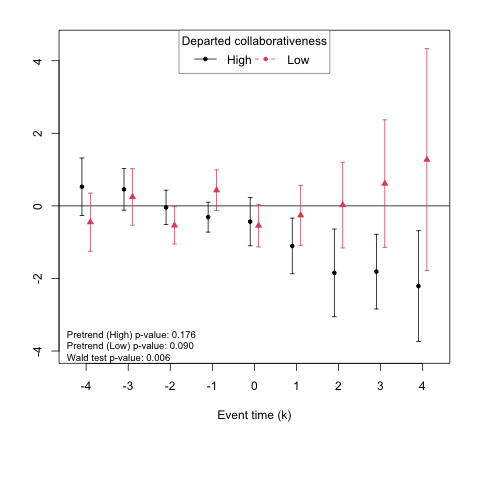
\includegraphics[width=\textwidth]{temp/output/collab/prs_opened_collab_cs_norm.png}
        \subcaption{By departed contributor collaborativeness}
        \label{fig:all_prs_opened_collab}
    \end{minipage}
    \caption{Impact of Key Contributor Departures on Project Outcomes}
    \label{fig:prs_opened}
\end{figure}

Figure~\ref{fig:prs_opened} presents results on how the departure of key contributors affects projects. Panel~\ref{fig:all_prs_opened} shows that projects experience statistically significant declines in the quantity of pull requests opened. These declines appear immediately following the departure and persist for two periods after. \todo[inline]{Discuss: what are the main takeaways? Project outcomes tend to trend upwards over time but imprecisely. Also, it's not mechanical} Panel~\ref{fig:all_prs_opened_collab} shows that post-departure project outcomes differ significantly depending on departed contributor collaborativeness. While projects where the departed contributor was collaborative are severely affected for several periods following the departure, projects where the departed contributor was uncollaborative are much less affected, particular in the long-term. 
\todo[inline]{What is the sd figure in quantity of PRs opened}
\todo[inline]{Align the axes to both be -2 to 2}
\todo[inline]{Systematize usage of "outcomes" over "activity"}

The results from Panel~\ref{fig:all_prs_opened_collab} are quite puzzling because the literature suggests that collaboration improves project-outcomes post departure.  \todo[inline]{Cite literature} For example, collaboration with the departed contributor prior to departure can help other contributors understand what the departed contributor's contributions were. This might, for instance, allow other contributors to react accordingly to make up the lost effort following a departure. 

One potential explanation of Panel~\ref{fig:all_prs_opened_collab} is that collaborative departed contributors might simultaneously be more involved with the project. If this were true, my comparison in Panel~\ref{fig:all_prs_opened_collab} would confound the impact of collaborative versus uncollaborative departed contributors with departed contributor involvement. I address whether this is a concern in the following figures. First, I examine how post-departure project outcomes vary by contributor involvement in Figure~\ref{fig:prs_opened_more_imp}. Then, I examine how collaboration interacts with contributor involvement to affect post-departure project outcomes in Figure~\ref{fig:prs_opened_inv_collab}
\todo[inline]{First, I should address whether it is true that collaborative departed contributors are more involved. Recall that mathematically the definition of collaboration is unrelated to the definition of involvement}

\begin{figure}[htbp]   
    \caption{Impact of Departed Importance on Organizational Outcomes} \label{fig:prs_opened_more_imp}
    \centering
    \begin{minipage}[b]{0.49\textwidth}
        \centering
        \subcaption{By problem involvement}    \label{fig:prs_opened_involved}
        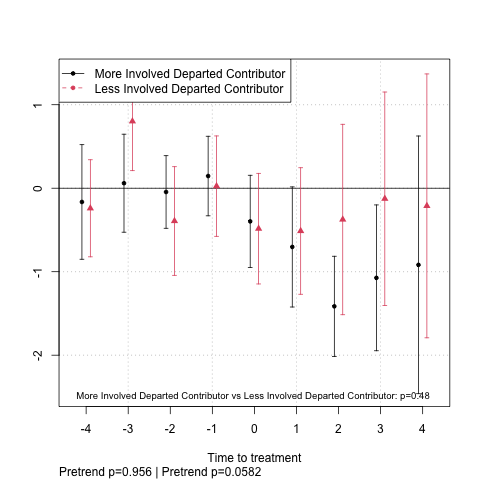
\includegraphics[width=\textwidth]{temp/output/collab/prs_opened_involved_cs_norm.png}
    \end{minipage}
    \begin{minipage}[b]{0.49\textwidth}
        \centering
        \subcaption{By PR opening involvement}    \label{fig:prs_opened_pr_involved}
        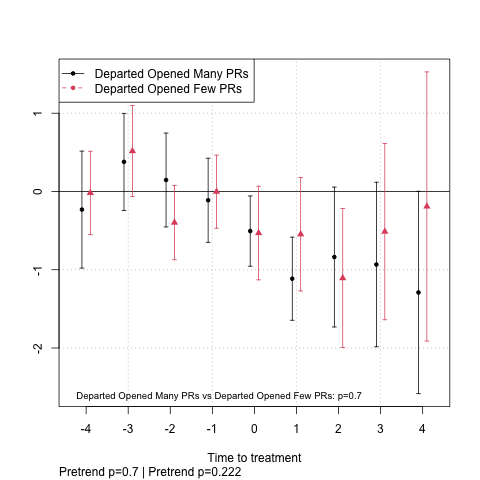
\includegraphics[width=\textwidth]{temp/output/collab/prs_opened_departed_opened_cs_norm.png}
    \end{minipage}
    \begin{minipage}[b]{0.49\textwidth}
        \centering
        \subcaption{More involved}    \label{fig:prs_opened_more_involved}
        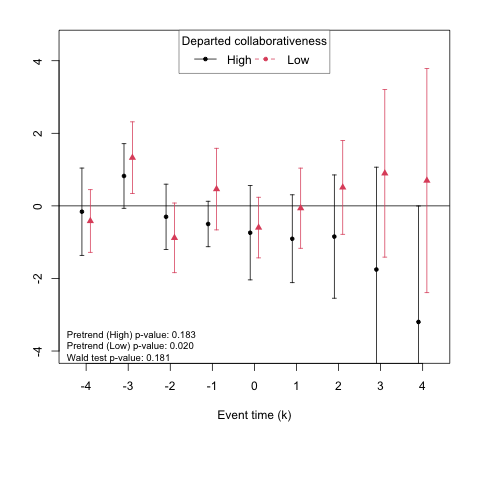
\includegraphics[width=\textwidth]{temp/output/collab_imp/inv0_cs_norm_prs_opened.png}
    \end{minipage}
    \begin{minipage}[b]{0.49\textwidth}
        \centering
        \subcaption{Less involved }    \label{fig:prs_opened_less_involved}
        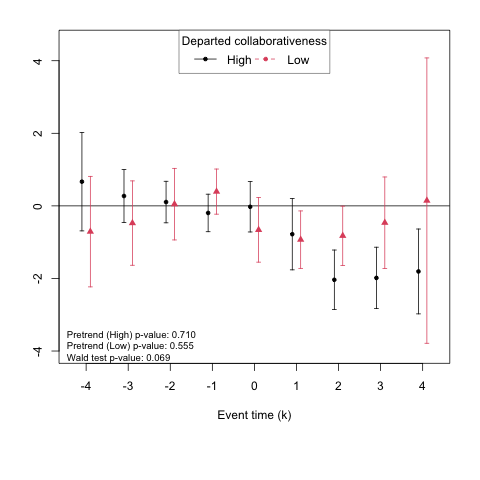
\includegraphics[width=\textwidth]{temp/output/collab_imp/inv1_cs_norm_prs_opened.png}
    \end{minipage}

  \begin{minipage}{1\textwidth}
    \textbf{Figure notes:} 
    Following Callaway and Sant’Anna (2021), I estimate event-study coefficients accompanied by 95\% simultaneous confidence bands. For each plot with event study estimates from two subsamples, I report three Wald-test p-values: one for the pretrend test in the first subsample, one for the pretrend test in the second subsample (both from Equation \ref{eq:wald_test_pretrends} in Section \ref{sec:main_method}), and one for the difference in treatment effects across subsamples (Equation \ref{eq:wald_test} in Section \ref{sec:att_subset}).  Panel~\subref{fig:prs_opened_involved}  subsets organizations by \textbf{departed member involvement}, as defined in Section~\ref{sec:org_level_subset}. Panel~\subref{fig:prs_opened_pr_involved}  subsets organizations by \textbf{departed member pull request involvement}, as defined in Section~\ref{sec:org_level_subset}. Panel~\subref{fig:prs_opened_more_involved} and Panel~\subref{fig:prs_opened_less_involved} condition on organizations where the departed was more and less involved by \textbf{departed member pull request involvement}, respectively and both subset by departed contributor collaborativeness
  \end{minipage}

\end{figure}

In Panel~\ref{fig:prs_opened_involved}, I find that while the departure of more involved contributors tends to affect projects more negatively, these effects are not statistically insignificant. This might be because my measure of departed involvement, which considers all problems, not just pull requests, is too broad. In Panel~\ref{fig:prs_opened_opened}, I divide projects by whether the departed contributor was historically more or less involved in opening pull requests. This comparison reveals statistically significant differences that align more with expectations. Projects where the departed contributor opened many pull requests experience statistically significant more severe declines than projects where the departed contributor opens few pull requests. In fact, these projects seem almost unaffected by departure. 
\todo[inline]{Describe effect stability over time}

Finally, in Panel~\ref{fig:prs_opened_involved_opened}, I examine how departed contributor involvement and pull request opening intensity interact to affect project outcomes. I find that project outcomes are most affected by departures where the departed was very involved in both problem solving and opening pull requests. Henceforth, refer to these as integral departed contributors. In contrast, departures by contributors who open many pull requests but are otherwise not very involved outside of that, or by contributors who are very involved in the project's problems but do not open many pull requests have statistically indistinguishable effects. Moreover, the effects incurred by their respective projects are comparatively minor and statistically indistinguishable from zero. The similarity in post-departure outcomesx between these two different project types suggests that in order to have a lasting impact on project pull request activity, a contributor needs to be heavily involved in both opening pull requests, and project discussion across all problem types. Only engaging in one or the other, as departed contributors in the aforementioned two types did, will not severely affect the project. 
\todo[inline]{I think I can do more work on the last few sentences of this paragraph to see if these findings are true - like are there actually ppl who are very involved in problem solving but just open few pull requests? }
\todo[inline]{Decide if I should describe the effects of everyone else (either the != != 1 group, or the ==0 ==0 group)}
\todo[inline]{Make axis scales the same, also find a way to quantify the difference between event study coefficients}
\todo[inline]{For right most plot, make the legend and coefficients seaprable + improve legend}
\todo[inline]{Feel like I can make the paragraph above smoother}

\begin{figure}[htbp]
    \centering
    % First row
    \begin{minipage}[b]{0.49\textwidth}
        \centering
        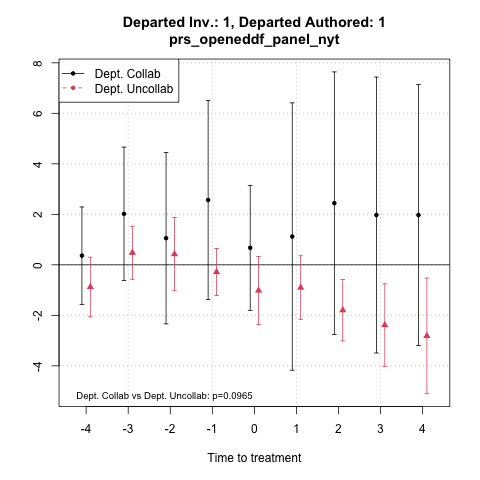
\includegraphics[width=\textwidth]{temp/output/collab_imp/auth1_inv1_cs_norm_prs_opened.png}
    \subcaption{Integral departed contributor}
    \label{fig:prs_opened_integral}
    \end{minipage}
    \hfill
    \begin{minipage}[b]{0.49\textwidth}
        \centering
        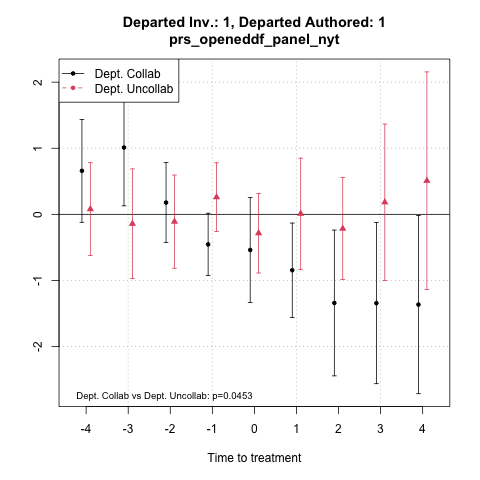
\includegraphics[width=\textwidth]{temp/output/collab_imp/auth_n1_inv_n1_cs_norm_prs_opened.png}
    \subcaption{Non-integral departed contributor}
    \label{fig:prs_opened_nonintegral}
    \end{minipage}

    
    \begin{minipage}[b]{0.32\textwidth}
        \centering
        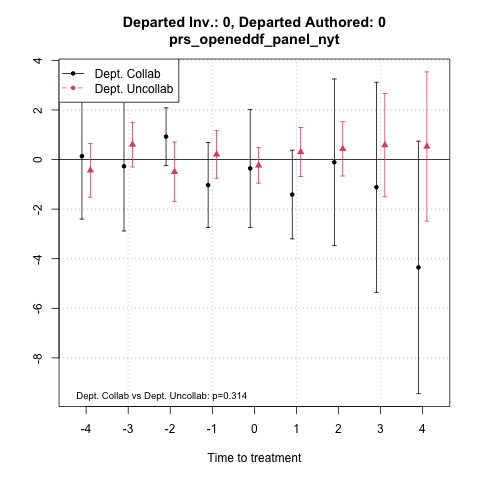
\includegraphics[width=\textwidth]{temp/output/collab_imp/auth0_inv0_cs_norm_prs_opened.png}
    \subcaption{Departed less involved, opened few PRs}
    \label{fig:prs_opened_noninv_nonopen}
    \end{minipage}
    \hfill
    \begin{minipage}[b]{0.32\textwidth}
        \centering
        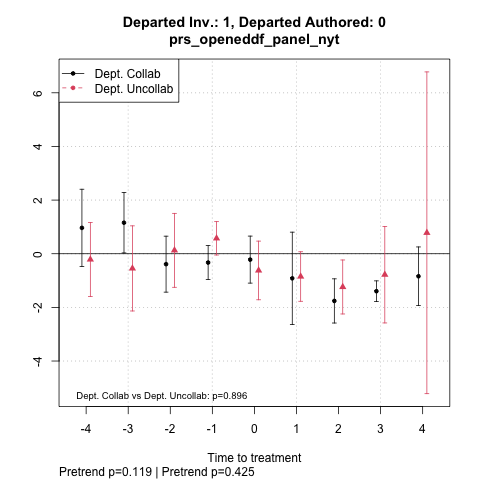
\includegraphics[width=\textwidth]{temp/output/collab_imp/auth0_inv1_cs_norm_prs_opened.png}
    \subcaption{Departed very involved, opened few PRs}
    \label{fig:prs_opened_inv_nonopen}
    \end{minipage}
    \hfill
    \begin{minipage}[b]{0.32\textwidth}
        \centering
        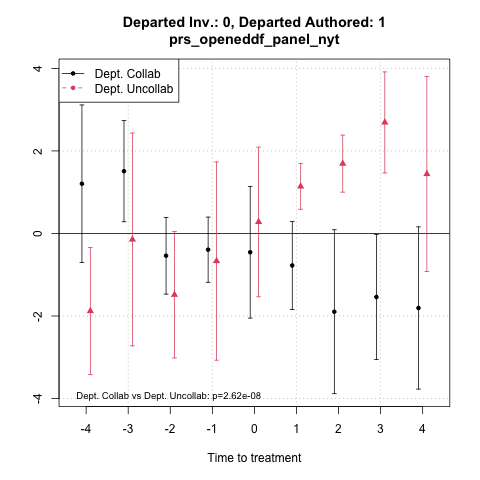
\includegraphics[width=\textwidth]{temp/output/collab_imp/auth1_inv0_cs_norm_prs_opened.png}
    \subcaption{Departed less involved, opened many PRs}
        \label{fig:prs_opened_nonvinv_open}

    \end{minipage}
    \caption{Departure Impact on Pull Requests Opened, by Departed Contributor Importance and Collaborativeness}
    \label{fig:prs_opened_inv_collab}
\end{figure}


Figure~\ref{fig:prs_opened_more_imp} tells us that departed contributor involvement does affect post-departure project outcomes. In Figure~\ref{fig:prs_opened_inv_collab}, I find that the nature of the departed contributor's involvement also affects the impact of collaboration with the departed contributor. 

In Panel~\ref{fig:prs_opened_integral}, I find that in projects with integral departed contributors, whether the departed contributor was collaborative or not determined whether projects avoided negative effects post-departure. The results from Panel~\ref{fig:prs_opened_integral} suggest that even when activity is heavily concentrated in the hands of one contributor, with collaboration, projects can overcome the ramifications of departures. When the departed contributor is not integral, Panel~\ref{fig:prs_opened_nonintegral} shows that uncollaborative projects tend to outperform collaborative projects, although the difference is not statistically significant. Results from aggregating non-integral departed contributors broadly extend to the 3 granular subcategories that make it up: the evidence from Panels~\ref{fig:prs_opened_noninv_nonopen}, \subref{fig:prs_opened_inv_nonopen} and \subref{fig:prs_opened_nonvinv_open} suggest that uncollaborative projects tend to outperform collaborative projects. 
\todo[inline]{This is also an interesting result - we'd expect collaboration to be less important}

\todo[inline]{How should I deal with the crazy 5 period point estimate}
\todo[inline]{Rename the bottom panel}
\todo[inline]{Improve the titles}
\todo[inline]{Change the axes to say Project-Specific Pull Request Standard Deviations or something shorter}


A project's outcomes are the product of the average outcome per contributor and the total quantity of contributors. I next examine how collaboration affects both, which will allow me to narrow down plausible mechanisms for collaboration's effect.


Let $Y_k$ be the outcome at time $k$ and $\bar Y_k$ be the average outcome per contributor at time $k$ and $N_k$ be the countributor count at time $k$. There's a slight abuse of notation because the expectation is over projects $i$ but I've ommitted $i$ from the terms. 
\begin{align*} 
  ATT_k &= \mathbb{E}\!\left[\frac{Y_k - \bar{Y}}{\sigma_Y}
             - \frac{Y_{-1} - \bar{Y}}{\sigma_Y}
             \Big| T=1\right] \\
           &= \mathbb{E}\!\left[\frac{Y_k - Y_{-1}}{\sigma_Y}
             \Big| T=1\right] \\
           &= \mathbb{E}\!\left[\frac{\bar{Y}_k N_k - \bar{Y}_{-1}N_{-1}}{\sigma_Y}
             \Big| T=1\right] \\
           &= \mathbb{E}\!\left[\frac{\bar Y_k (N_k - N_{-1})}{\sigma_Y}
             + \frac{(\bar Y_k - \bar Y_{-1}) N_{-1}}{\sigma_Y}
             \Big| T=1\right]
\end{align*}
Empirically, I can estimate both of the following expressions, which allows me to characterize how changes in the average and contributor count affect the outcome. 


\begin{figure}[htbp]
    \centering
    \begin{minipage}[b]{0.49\textwidth}
        \centering
        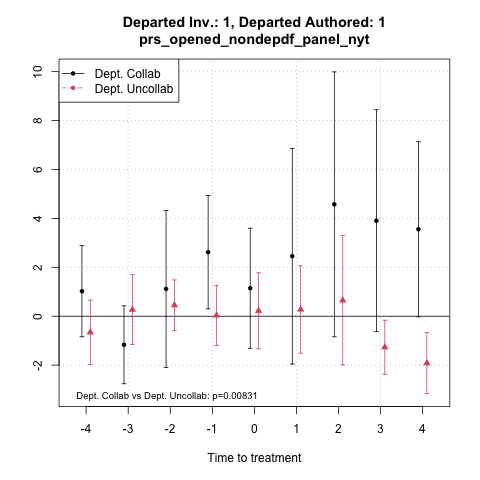
\includegraphics[width=\textwidth]{temp/output/collab_imp/auth1_inv1_cs_norm_prs_opened_nondep.png}
    \subcaption{All contributors except the departed}
    \label{fig:prs_opened_nondep}
    \end{minipage}
    \hfill
    \begin{minipage}[b]{0.49\textwidth}
        \centering
        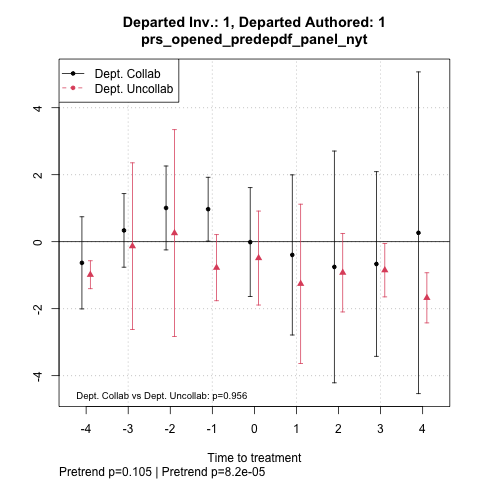
\includegraphics[width=\textwidth]{temp/output/collab_imp/auth1_inv1_cs_norm_prs_opened_predep.png}
    \subcaption{All contributors present prior to departure}
    \label{fig:prs_opened_predep}
    \end{minipage}
    \hfill
    \begin{minipage}[b]{0.49\textwidth}
        \centering
        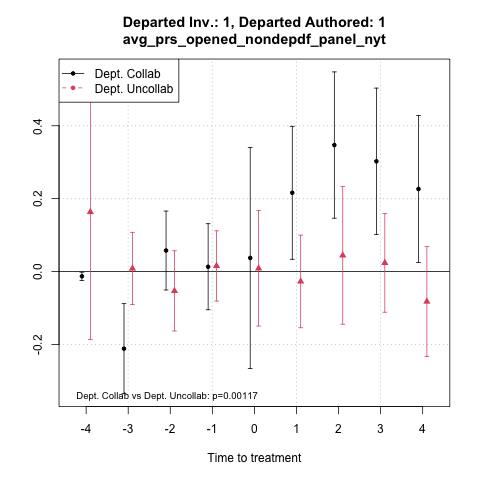
\includegraphics[width=\textwidth]{temp/output/collab_imp/auth1_inv1_cs_norm_avg_prs_opened_nondep.png}
    \subcaption{Average PRs opened, all but departed}
    \label{fig:avg_prs_opened_nondep}

    \end{minipage}
    \hfill
    \begin{minipage}[b]{0.49\textwidth}
        \centering
        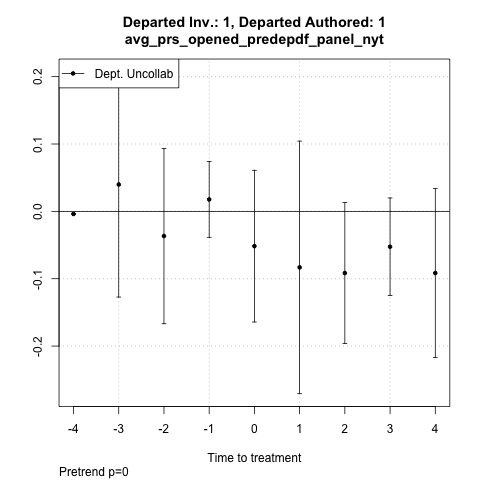
\includegraphics[width=\textwidth]{temp/output/collab_imp/auth1_inv1_cs_norm_avg_prs_opened_predep.png}
    \subcaption{Average PRs opened, contributors present pre-departure}
    \label{fig:avg_prs_opened_predep}
    \end{minipage}
    \hfill
    \begin{minipage}[b]{0.49\textwidth}
        \centering
        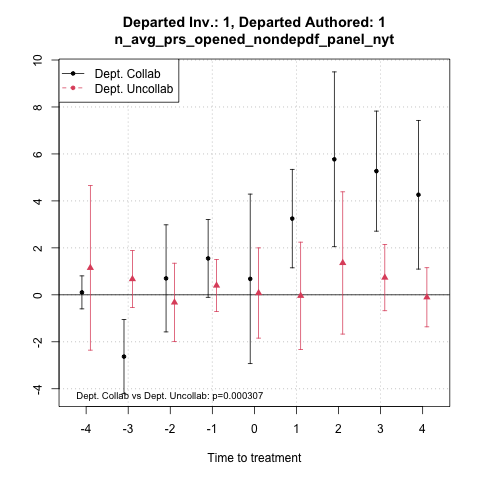
\includegraphics[width=\textwidth]{temp/output/collab_imp/auth1_inv1_cs_norm_n_avg_prs_opened_nondep.png}
    \subcaption{Impact of changes in average, all but departed}
    \label{fig:impact_avg_prs_opened_nondep}
    \end{minipage}
    \hfill
    \begin{minipage}[b]{0.49\textwidth}
        \centering
        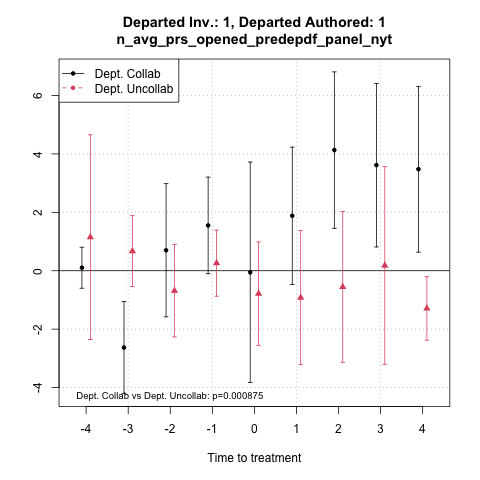
\includegraphics[width=\textwidth]{temp/output/collab_imp/auth1_inv1_cs_norm_n_avg_prs_opened_predep.png}
    \subcaption{Impact of changes in average, contirbutors present pre-departure}
    \label{fig:impact_avg_prs_opened_predep}

    \end{minipage}
    \caption{Integral Departure Impact on Average Outcomes and Participation}
\end{figure}


I make a few modifications to the sample. First, in the raw outcome count, all problems where the departed contributor was involved in were excluded. 

I exclude all pull requests the departed contributor was involved in because I'm interested in how contributors other than the departed react to departure. Including the departed contributor in the calculation of the average would prevent me from discerning changes in average activity post-departure caused by the loss of the departed or changes in behavior by other contributors. 

Finally, the denominator in my average is the total number of contributors, across all aspects of the project, except for the departed contributor. I use this denominator as opposed to something like the number of people who open pull requests because I want to account for changes along the extensive margin (whether people open pull requests) and along the intensive margin (conditional on opening one pull request, how many they open). 

Panels~\subref{fig:prs_opened_nondep}, ~\subref{fig:avg_prs_opened_nondep}, ~\subref{fig:impact_avg_prs_opened_nondep} all use the sample of pull requests that exclude activity that the departed contributor was involved in. Panels~\subref{fig:prs_opened_nondep} shows that in projects where the departed contributor was integral, the quantity of pull requests opened by all other contributors rises in the period following departure. Panel~\subref{fig:avg_prs_opened_nondep} replaces the outcome with the standardized average quantity of pull requests opened. We see in Panel~\subref{fig:avg_prs_opened_nondep} that the rise in Panel~\subref{fig:prs_opened_nondep} is driven by increases in average activity per contributor. Finally, in Panel~\subref{fig:impact_avg_prs_opened_nondep}, we see that the effect of the increase in average on the quantity of pull requests opened accounts for almost the entire effect.
\todo[inline]{Perhaps replace panel E with a barplot showing what \% of the change is due to which factor}


I also show the effect of contributor departures on the average activity of all individuals who had first participated in the project prior to the departure. This subset is of particular interest because they are the most likely beneficiaries of collaboration. 
Panels~\subref{fig:prs_opened_predep}, ~\subref{fig:avg_prs_opened_predep}, ~\subref{fig:impact_avg_prs_opened_predep} mirror the previous analysis except that we replace outcomes with a version that also excludes contributions by contributors who first participated prior to the contributor's departure. These are individuals who are most plausibly benefited by the contributor's departure, as the most direct effect of collaboration is probably on the people who are working with you. I find the same qualitative results. \textbf{One noteworthy point is that the point estimates when outcomes are averages decrease when we exclude new contributors, which suggests that new contributors are just as productive, if not more productive at opening pull requests than existing contributors on a per-capita basis. This is quite interesting and merits further exploration.}



\todo[inline]{Should I characterize the intensive vs. extensive margin?}
$\bar Y_{k}^{!0} $ is average outcome among only individuals whose individual outcome exceeded 0 in period $k$. Let $p_k^{!0}$ be the proportion of individuals in period $k$ whose individual outcome exceeds 0. 
\begin{align*}
    \mathbb{E}\!\left[\frac{(\bar Y_k - \bar Y_{-1}) }{\sigma_Y} \Big| T=1\right] &= \mathbb{E}\!\left[\frac{ \bar Y_{k}^{!0}  p_k^{!0} - \bar Y_{-1}^{!0} p_{-1}^{!0} }{\sigma_Y} \Big| T=1\right] \\
    &=  \mathbb{E}\!\left[\frac{ \bar  Y_{k}^{!0}  p_k^{!0} - \bar  Y_{k}^{!0} p_{-1}^{!0} +\bar Y_{k}^{!0}  p_{-1}^{!0}  -\bar Y_{-1}^{!0}  p_{-1}^{!0} }{\sigma_Y} \Big| T=1\right] \\
    &=  \mathbb{E}\!\left[\frac{ \bar  Y_{k}^{!0} \left(p_k^{!0} -  p_{-1}^{!0}  \right) +  \left( \bar  Y_{k}^{!0}  - \bar Y_{-1}^{!0} \right)  p_{-1}^{!0}  }{\sigma_Y} \Big| T=1\right]
\end{align*}
\todo[inline]{Estimate, ideally it's mostly intensive not extensive margin}

\begin{figure}[htbp]
    \centering
    \begin{minipage}[b]{0.49\textwidth}
        \centering
        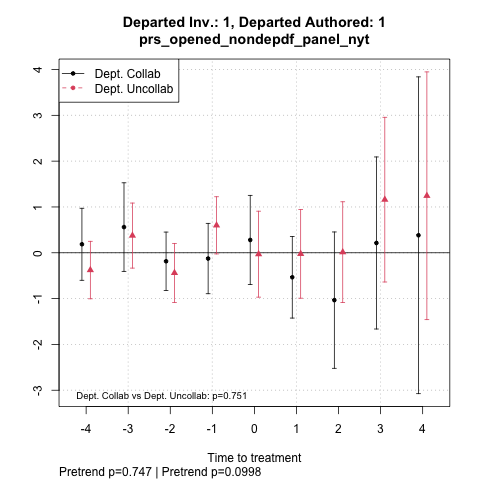
\includegraphics[width=\textwidth]{temp/output/collab_imp/auth_n1_inv_n1_cs_norm_prs_opened_nondep.png}
    \subcaption{All contributors except the departed}
    \end{minipage}
    \hfill
    \begin{minipage}[b]{0.49\textwidth}
        \centering
        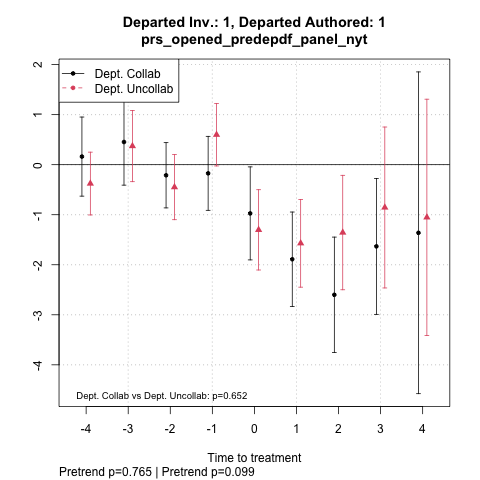
\includegraphics[width=\textwidth]{temp/output/collab_imp/auth_n1_inv_n1_cs_norm_prs_opened_predep.png}
    \subcaption{All contributors present prior to departure}
    \end{minipage}
    \hfill
    \begin{minipage}[b]{0.49\textwidth}
        \centering
        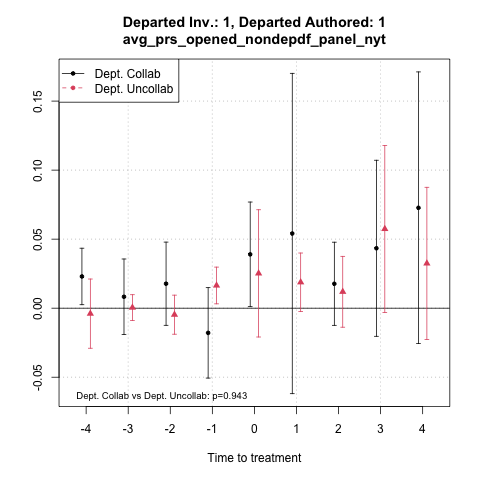
\includegraphics[width=\textwidth]{temp/output/collab_imp/auth_n1_inv_n1_cs_norm_avg_prs_opened_nondep.png}
    \subcaption{Average PRs opened, all but departed}
    \end{minipage}
    \hfill
    \begin{minipage}[b]{0.49\textwidth}
        \centering
        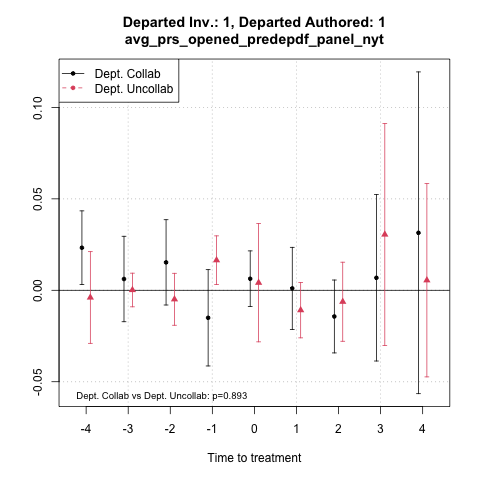
\includegraphics[width=\textwidth]{temp/output/collab_imp/auth_n1_inv_n1_cs_norm_avg_prs_opened_predep.png}
    \subcaption{Average PRs opened, contributors present pre-departure}
    \end{minipage}
    \hfill
    \begin{minipage}[b]{0.49\textwidth}
        \centering
        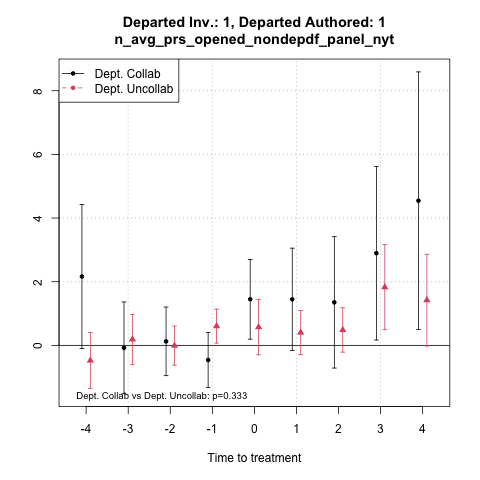
\includegraphics[width=\textwidth]{temp/output/collab_imp/auth_n1_inv_n1_cs_norm_n_avg_prs_opened_nondep.png}
    \subcaption{Impact of changes in average, all but departed}
    \end{minipage}
    \hfill
    \begin{minipage}[b]{0.49\textwidth}
        \centering
        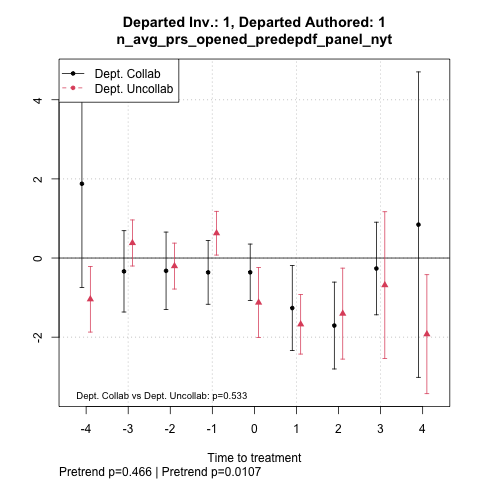
\includegraphics[width=\textwidth]{temp/output/collab_imp/auth_n1_inv_n1_cs_norm_n_avg_prs_opened_predep.png}
    \subcaption{Impact of changes in average, contirbutors present pre-departure}
    \end{minipage}
    \caption{Integral Departure Impact on Average Outcomes and Participation}
\end{figure}

\todo[inline]{also do barplots for bottom row}
\todo[inline]{takeaway is that it's caused by departures not changes in the average which is interesting. Should I dig into more why people leave? (technically 2 todos ig) }

\subsection{Mechanisms behind collaboration's effect}
\todo[inline]{Notes on other collaboration:\\
- Correlation between departed collaborative score and other collaborative score\\
- Binned event study with other collaborative\\
- Binned event study with other collaborative, focusing on integral vs. non-integral departures
}


\begin{figure}[htbp]
    \centering
    \begin{minipage}[b]{0.32\textwidth}
        \centering
        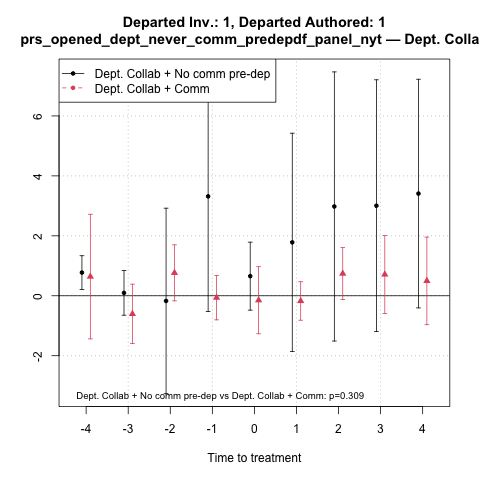
\includegraphics[width=\textwidth]{temp/output/collab_imp/auth1_inv1_cs_norm_prs_opened_dept_never_comm_predep_Dept.Collab.png}
    \subcaption{Communicators vs. Non-communicators, Collaborative Projects, integral departures}
    \label{fig:prs_opened_comm_collab_int_predep}
    \end{minipage}
    \hfill
    \begin{minipage}[b]{0.32\textwidth}
        \centering
        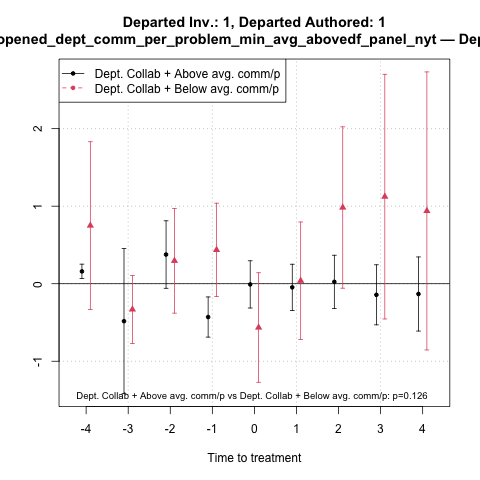
\includegraphics[width=\textwidth]{temp/output/collab_imp/auth1_inv1_cs_norm_prs_opened_dept_comm_per_problem_min_avg_above_Dept.Collab.png}
    \subcaption{Above vs. Below avg. communicators/problem, Collaborative Projects, integral departures}
    \label{fig:prs_opened_comm_collab_per_int}
    \end{minipage}
    \hfill
        \begin{minipage}[b]{0.32\textwidth}
        \centering
        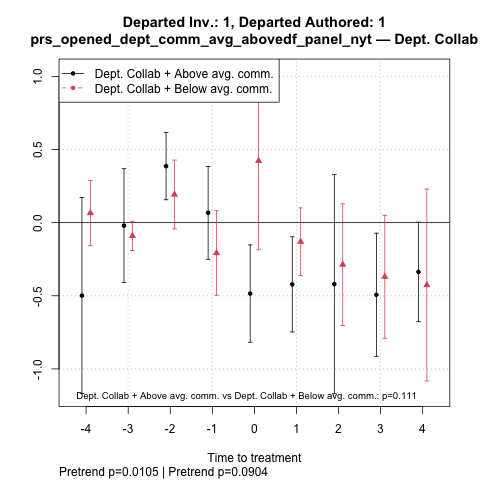
\includegraphics[width=\textwidth]{temp/output/collab_imp/auth1_inv1_cs_norm_prs_opened_dept_comm_avg_above_Dept.Collab.png}
    \subcaption{Above vs. Below avg. communicators, Collaborative Projects, integral departures}
    \label{fig:prs_opened_comm_collab_comm_int}
    \end{minipage}


    \begin{minipage}[b]{0.32\textwidth}
    \centering
    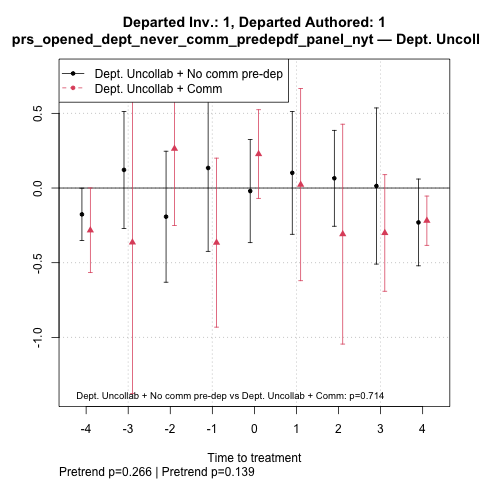
\includegraphics[width=\textwidth]{temp/output/collab_imp/auth1_inv1_cs_norm_prs_opened_dept_never_comm_predep_Dept.Uncollab.png}
    \subcaption{Communicators vs. Non-communicators, Uncollaborative Projects, integral departures}
    \label{fig:prs_opened_comm_uncollab_int_predep}
    \end{minipage}
    \hfill
    \begin{minipage}[b]{0.32\textwidth}
        \centering
        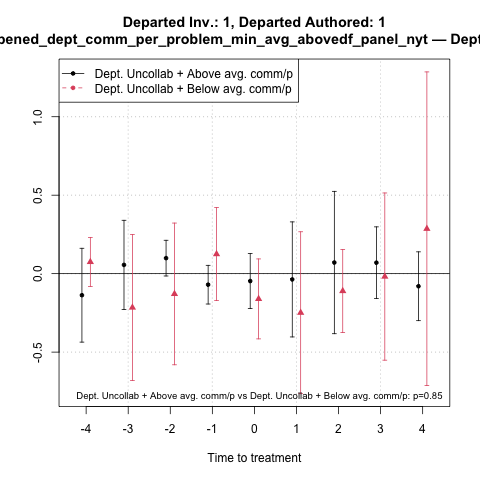
\includegraphics[width=\textwidth]{temp/output/collab_imp/auth1_inv1_cs_norm_prs_opened_dept_comm_per_problem_min_avg_above_Dept.Uncollab.png}
    \subcaption{Above vs. Below avg. communicators/problem, Uncollaborative Projects, integral departures}
    \label{fig:prs_opened_comm_uncollab_per_int}
    \end{minipage}
    \hfill
        \begin{minipage}[b]{0.32\textwidth}
        \centering
        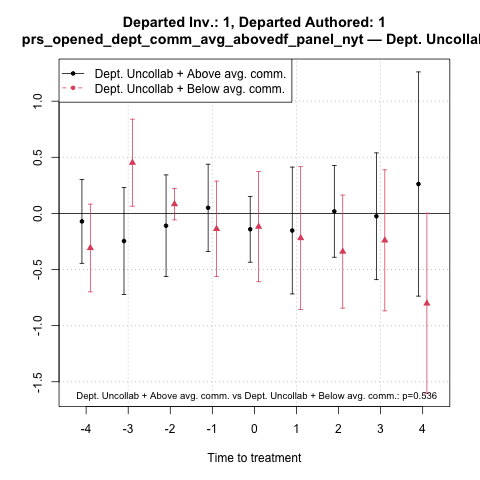
\includegraphics[width=\textwidth]{temp/output/collab_imp/auth1_inv1_cs_norm_prs_opened_dept_comm_avg_above_Dept.Uncollab.png}
    \subcaption{Above vs. Below avg. communicators, Uncollaborative Projects, integral departures}
    \label{fig:prs_opened_comm_uncollab_comm_int}
    \end{minipage}
    \caption{Impact of Communication on Post-Departure Outcomes in Projects with Integral Departures}
    \label{fig:prs_opened_comm}
\end{figure}


In projects where the departed contributor was integral
\begin{itemize}
    \item Collaborative departed contributors: non-communicators (present prior to departure) whose activity rises, communicators are uanffected
    \item Uncollaborative departed contributors: no difference between communicators/non-communicators, activity declines
\end{itemize}
Eventually: incorporate dynamics of average vs. people leaving, it's not super clear to me right now what the primary mechanism is. \\
Now, consider the intensive margin of communication - only for collaborative projects, doesn't matter for uncollaborative projects:
\begin{itemize}
    \item it SEEMS like along the intensive margin, communicating less per problem helps??
    \item it also seems like along the intensive margin, communicating MORE helps
\end{itemize}

\begin{figure}[htbp]
    \centering
    \begin{minipage}[b]{0.24\textwidth}
        \centering
        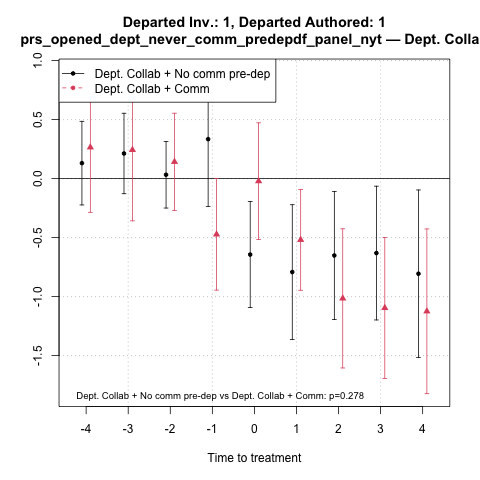
\includegraphics[width=\textwidth]{temp/output/collab_imp/auth_n1_inv_n1_cs_norm_prs_opened_dept_never_comm_predep_Dept.Collab.png}
    \subcaption{Communicators vs. Non-communicators, Collaborative Projects, integral departures}
    \label{fig:prs_opened_comm_collab_nonint_predep}
    \end{minipage}
    \hfill
    \begin{minipage}[b]{0.24\textwidth}
        \centering
        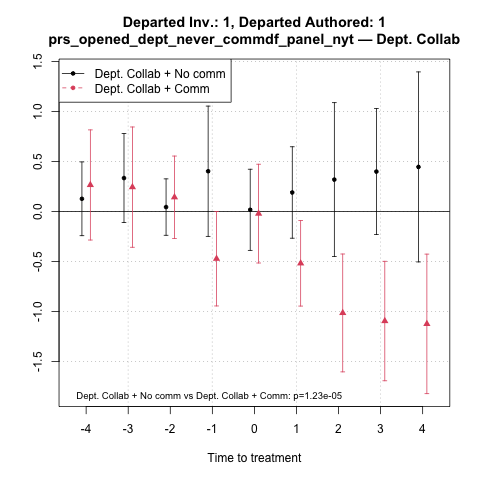
\includegraphics[width=\textwidth]{temp/output/collab_imp/auth_n1_inv_n1_cs_norm_prs_opened_dept_never_comm_Dept.Collab.png}
    \subcaption{Communicators vs. Non-communicators, Collaborative Projects, integral departures, include newcomers}
    \label{fig:prs_opened_comm_collab_nonint}
    \end{minipage}
    \hfill
    \begin{minipage}[b]{0.24\textwidth}
        \centering
        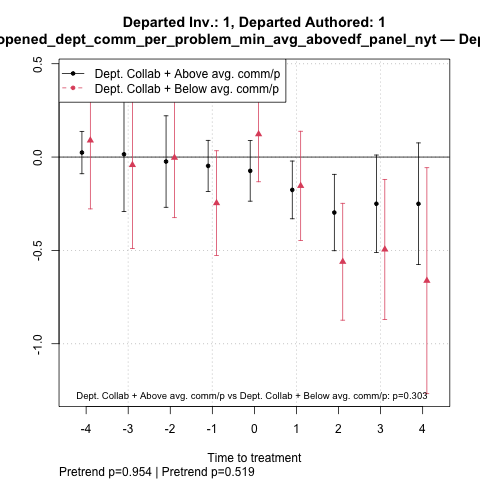
\includegraphics[width=\textwidth]{temp/output/collab_imp/auth_n1_inv_n1_cs_norm_prs_opened_dept_comm_per_problem_min_avg_above_Dept.Collab.png}
    \subcaption{Above vs. Below avg. communicators/problem, Collaborative Projects, integral departures}
    \label{fig:prs_opened_comm_collab_per_nonint}
    \end{minipage}
    \hfill
        \begin{minipage}[b]{0.24\textwidth}
        \centering
        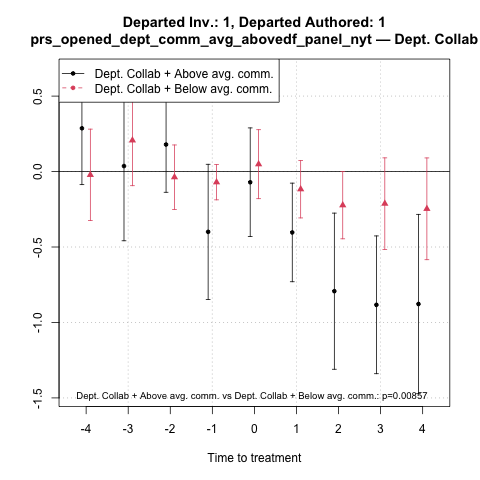
\includegraphics[width=\textwidth]{temp/output/collab_imp/auth_n1_inv_n1_cs_norm_prs_opened_dept_comm_avg_above_Dept.Collab.png}
    \subcaption{Above vs. Below avg. communicators, Collaborative Projects, integral departures}
    \label{fig:prs_opened_comm_collab_comm_nonint}
    \end{minipage}


    \begin{minipage}[b]{0.24\textwidth}
    \centering
    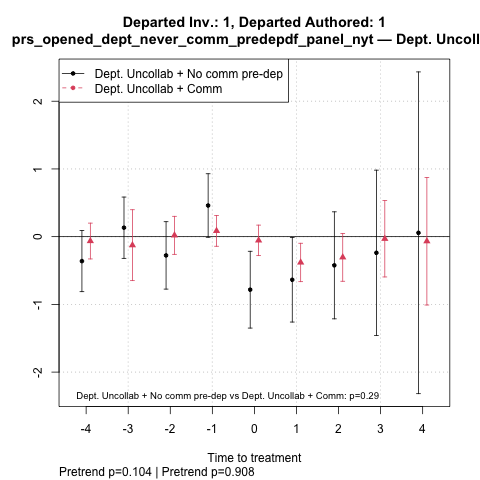
\includegraphics[width=\textwidth]{temp/output/collab_imp/auth_n1_inv_n1_cs_norm_prs_opened_dept_never_comm_predep_Dept.Uncollab.png}
    \subcaption{Communicators vs. Non-communicators, Uncollaborative Projects, integral departures}
    \label{fig:prs_opened_comm_uncollab_nonint_predep}
    \end{minipage}
    \hfill
    \begin{minipage}[b]{0.24\textwidth}
        \centering
        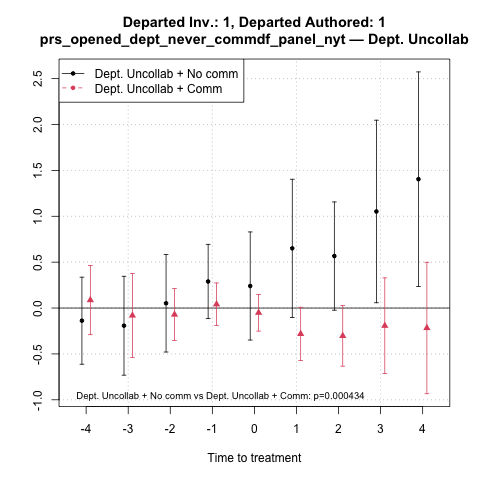
\includegraphics[width=\textwidth]{temp/output/collab_imp/auth_n1_inv_n1_cs_norm_prs_opened_dept_never_comm_Dept.Uncollab.png}
    \subcaption{Communicators vs. Non-communicators, Unollaborative Projects, integral departures, include newcomers}
    \label{fig:prs_opened_comm_collab_nonint}
    \end{minipage}
    \hfill
    \begin{minipage}[b]{0.24\textwidth}
        \centering
        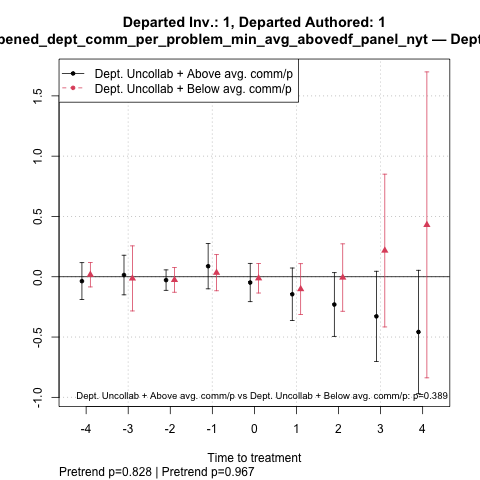
\includegraphics[width=\textwidth]{temp/output/collab_imp/auth_n1_inv_n1_cs_norm_prs_opened_dept_comm_per_problem_min_avg_above_Dept.Uncollab.png}
    \subcaption{Above vs. Below avg. communicators/problem, Uncollaborative Projects, integral departures}
    \label{fig:prs_opened_comm_uncollab_per_nonint}
    \end{minipage}
    \hfill
        \begin{minipage}[b]{0.24\textwidth}
        \centering
        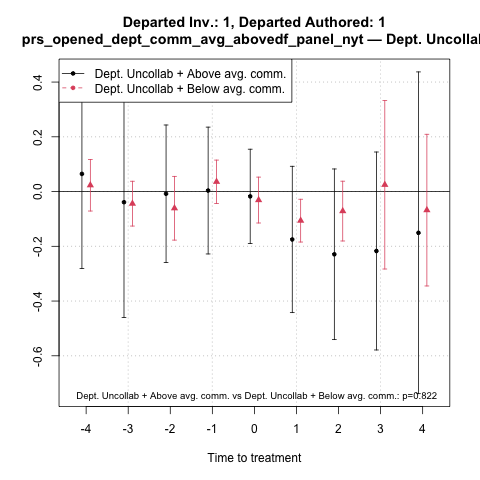
\includegraphics[width=\textwidth]{temp/output/collab_imp/auth_n1_inv_n1_cs_norm_prs_opened_dept_comm_avg_above_Dept.Uncollab.png}
    \subcaption{Above vs. Below avg. communicators, Uncollaborative Projects, integral departures}
    \label{fig:prs_opened_comm_uncollab_comm_nonint}
    \end{minipage}
    \caption{Impact of Communication on Post-Departure Outcomes in Projects with Integral Departures}
    \label{fig:prs_opened_comm}
\end{figure}


In projects where the departed contributor was not integral
\begin{itemize}
    \item Communication makes no difference in collaborative vs. uncollaborative projects - both are negatively affected. 
    \item New contributors do make a HUGE difference
\end{itemize}

Now, consider the intensive margin of communication.
\begin{itemize}
    \item Communicating more per problem in collaborative projects has no effect, which is the same as in integral departures. However, unlike in integral departures, communciating less per problem has the opposite effect - it worsens things for collaborative projects
    \item Communicating less has no effect, which is the same as in integral departures, but communicating more worsens things for collaborative projects 
\end{itemize}

\todo[inline]{Think about what makes integral vs. non integral departures different, and why that causes the effects below. I think the solution is to examine the averages to see whether there are actually contradicting effects/what the dynamcis 
1. Non-communicators much better off compared to communicators in integral projects, but not in nonintegral projects
2. Low intensity/high breadth communicators better off in integral projects whereas high intensity/low breadth communicators are better off in integral projects
}

\todo[inline]{
What about if we focus on the specific contributors that we had designated their "key collaborators"
}

\todo[inline]{Execute tests of whether they're learning}

\todo[inline]{Characterize tradeoffs
1. Do collaborative and uncollaborative projects differ in productivity?\\
2. Do collaborative and uncollaborative projects differ in the total number of discussants present per problem? \\
3. Does collaborative and uncollaborative projects differ in how much time it takes to close a PR/issue? \\

4. What are the implications of having more discussants/reviewers?\\
- When review comments are made, how much additional change (code-wise) is needed (additional commits, LOC changed etc)? \\
- Are more discussants associated with more comments, longer closing time? We can also look at first comment time and define closing time as last - first comment time. \\
- How much time occurs between each comment? \\
- Can use project/time/project-time fixed effects in a regression\\
}
\todo[inline]{Bring in the bin scatter for downstream outcomes...}

\todo[inline]{Clean up everything below}
\todo[inline]{Other thought (NEED TO THINK ABOUT HOW THIS RELATES TO PAPER THEME): Are these problems still subject to the same level of review (unchanged quantity of pr review comments per PR) post-departure?}

\textbf{Other ways of splitting the data}
\begin{enumerate}
    \item How does the effect of fast vs. slow communication affect the effect of collaboration
\end{enumerate}
\textbf{Other outcomes to consider}
\begin{itemize}
    \item Are they linking issues to PRs at higher rates or closing issues at lower rates?
    \item D\textbf{oes their language evolve to be more similar to the departed's?}
    \item Do they solve problems that are outside of their realm (using issue tags or language similarity)?
\end{itemize}
    
\begin{enumerate}
    \item \textbf{RANT}
    \item How does collaboration allow contributors to increase their average activity? What do collaborative projects possess that uncollaborative projects don't?\\
    \textbf{In my ideal paper, I would be able to say: here are three ways collaboration affect projects. 1) Collaboration's positive benefit is directly related to how much communication and information flow occurred - contributors who communicated most or had collaborated longest (controlling for tenure) with the departed see their overall activity increase and also start solving problems in areas they were unfamiliar with that the departed was. That this only occurs when communication is a back and forth and not when they're independently working on the same issue at different time periods. 2) In contrast, collaboration doesn't benefit projects where the departed contributor was less involved - this is why and here's how we know those results are legit, why is this interesting etc. Finally, collaboration isn't a magic wand - here are some of the costs of collaboration pre-departure}
\end{enumerate}

    
Once I do that, I think I will be in a state to determine whether I want to either a) spend time writing everything up as a first draft or b) do additional robsutness/analysis/write up a model before I write up the draft

\todo[inline]{Show robsutness using periods other than 5 pre periods once I figure out the final statistic}
\todo[inline]{Show results}
\begin{enumerate}
    \item Takeaway from logs with zeros is to levels and normalize, or to normalize outcomes by a reasonable measure.
    \item Takeaway from AER:I Abadie is that nonsignificant results with interesting confidence intervals should also be covered. 
\end{enumerate}

\todo[inline]{\href{https://www.jonathandroth.com/assets/files/roth_pretrends_testing.pdf}{Check Roth for pretrends testing}}
\todo[inline]{Rule out the easy confounders/explanations first before dividing into more interesting explanations}
What I'm hoping to establish next is whether/the degree to which the decline in PRs is mechanical

\textbf{Can I turn these into robustness checks?}
\begin{enumerate}
    \item Am I confounding the effect of how collaborative the departed contributor is with how important/involved the departed contributor is? 
    \todo[inline]{Explain that because the denominator on departed contributor involvement is the \# of questions the departed is involved in, there's no mechanical relationship between departed contributor involvement and collaboration}
    \todo[inline]{Examine what happens when I split by departed contributor importance. I can do this by calculating departed involvement as the proportion of problems they're involved in, and comparing event study results for the more/less involved bins x collaboration. I should also examine how things vary by more/less involved bins. I expect there to be a difference based off the more/less involved bins - I don't know what I will see when I interact collaboration with the results. }
    \textcolor{blue}{Note: calculations done, called "departed\_involved\_2bin"}
    \item How does collaborative score vary by 
    \begin{enumerate}
        \item Key contributor count \textcolor{blue}{"key\_contributor\_count\_2bin"}
        \item Total contributor count \textcolor{blue}{"total\_contributor\_count\_2bin"}
        \item Problem count \textcolor{blue}{"problem\_count\_2bin"}
    \end{enumerate}
    and how do each of the factors above interact with collaborative score in determining the outcome? For the last two consider how size is related to the proportion/count difference. 
    \todo[inline]{Execute the task above. Definitions should be straightforward}
    \item What is the effect of collaboration among other contributors (No effect). Might the presence of prior collaboration among other contributors have an effect depending on how collaborative the departed contributor was? 
    \todo[inline]{Describe in more detail results for other collaboration}
    \todo[inline]{Execute the task above. One hypothesis is that other collaboration is only helpful when the departed contributor was collaborative and task allocation is required. This is because other departed contributors now need to reallocate what tasks they are working on to account for the departed's loss, but this reallocation only happens if there's collaboration with the deprated $\iff $ responsibiltiies can easily be reallocated}
    \item Departed contributors can affect whether PRs are opened in two ways: By opening PRs themselves/authoring the majority of the commits involved in the PR, or by contributing to discussion that leads to PRs being opened. Can I identify how active departed contributors are in each and see
    \begin{enumerate}
        \item Whether the discussion mechanism has any effect on post-departure outcomes
        \item How both factors interact with collaboration (Expect collaboration to interact with discussion in more interesting ways)
    \end{enumerate}
    \todo[inline]{Execute the above. 1) Does the effect of departed involvement change when we also vary by PR opening intensity (test 2 variations of opening PRs: one that excludes non-opening/commit involvement in PRS and one that does), 2) How does collaboration interact with PR opening intensity to affect outcomes, 3) What's the best way to loop departed involvement in as well - answer will be easier after I know 1}
    \textcolor{blue}{Note: Calculated prop of PRs opened/authored by departed, out of all the author is involved in. Note that the denominator is all PRs implemented by the departed not all PRs implemented by the project. If I had the denominator be total problems, I wouldn't be able to differentiate, holding departed involvement constant, projects with high/low departed involvement because then the lower bound of departed PR opening would be mechanically increasing in departed PR involvement}
    \textbf{complicated}
    

    \item Mass departures in collaborative projects, is there a systematic proximity to release in either

    \item There's a persistent (and a decrease) in PRs opened over time, so it's not just that projects have been abandoned. What's driving this? Are people able to somewhat wrap up problems that the departed was involved in?
    \item \textbf{What is their role as a collaborator?}
    
\end{enumerate}

\textbf{Robustness}
\begin{enumerate}
    \item What do development related characteristics look like prior to departure? I'm trying to see if I can provide quantitative evidence of "no anticipation" in that behavior across a wide range of measures is unchanged
\end{enumerate}

\section{Conclusion} \label{sec:conclusion}



\singlespacing


\clearpage

\onehalfspacing

\section*{Tables} \label{sec:tab}
\addcontentsline{toc}{section}{Tables}



\clearpage

\section*{Figures} \label{sec:fig}
\addcontentsline{toc}{section}{Figures}

%\begin{figure}[hp]
%  \centering
%  \includegra\phics[width=.6\textwidth]{../fig/placeholder.pdf}
%  \caption{Placeholder}
%  \label{fig:placeholder}
%\end{figure}




\clearpage

\section*{Appendix A. Placeholder} \label{sec:appendixa}
\addcontentsline{toc}{section}{Appendix A}


\end{document}